%!TEX root = ./trampoline.tex

\chapter{Ports details}

\section{PowerPC}

\subsection{The MPC5510 Memory Protection Unit}

The access control rights of the memory region descriptor rules the access of 5 bus masters (labeled from 4 to 0). Unused bus masters are set to the same access right for all the regions. Bus master 4 is used for factory testing only, so the access rights should be set to no access. Bus master 3 is the Flexray controller. Since it is not used in the current version of Trampoline, it is set to no access to. Bus master 2 is the DMA controller. For the same reason it is set to no access. Bus master 1 is the Z0 core. Again it is set to no access.

The access control rights register has the following bit usage:

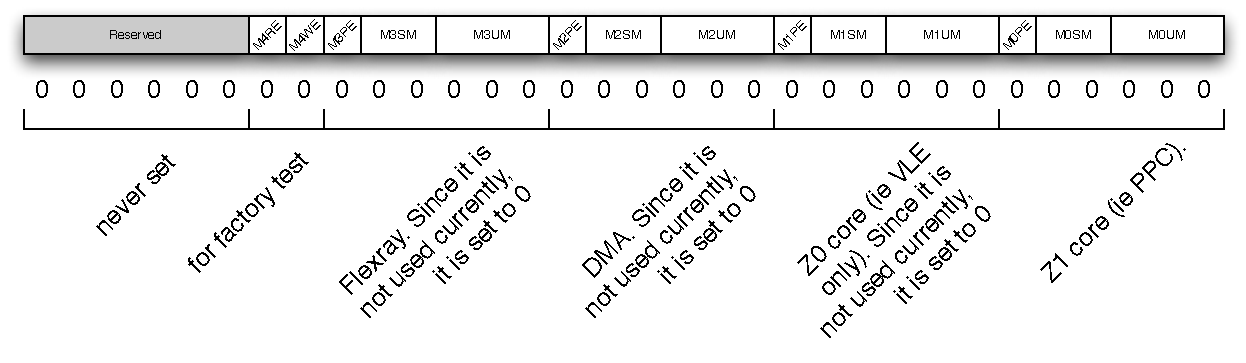
\includegraphics[width=\textwidth]{pictures/MPUacr.pdf} 

Bus master 4 is a special case. The 2 bits have the following meaning:

\rowcolors{1}{white}{light-gray}
\begin{longtableii}{p{0.4in}|p{4.8in}}{}{Bit}{Meaning}
  \lineii{M4RE}
  {If set to 1, bus master 4 may \strong{read} memory in the region. If 0, no read is allowed}
  \lineii{M4WE}
  {If set to 1, bus master 4 may \strong{write} memory in the region. If 0, no write is allowed}
\end{longtableii}

So in our case, these bits are set to 0.

Of course, other bus masters have more sophisticated access right:

\rowcolors{1}{white}{light-gray}
\begin{longtableii}{p{0.4in}|p{4.8in}}{}{Bit}{Meaning}
  \lineii{MxPE}
  {The PID Enable bit. Set to 0 in our case}
  \lineii{MxSM}
  {These 2 bits rules the supervisor mode access control with the following meaning: $00=rwx$, $01=rx$, $10=rw$, $11=$ {\it same as defined by MxUM}. In our case, it is set to $00$ for code and constants and to $11$ for data.}
  \lineii{MxUM}
  {These 2 bits rules the user mode access control. The first bit means $r$, the second one $w$ and the third one $x$.}
\end{longtableii}

Trampoline uses 4 descriptors:

\rowcolors{1}{white}{light-gray}
\begin{longtableiii}{p{0.8in}|p{2in}|p{2.3in}}{}{Descriptor}{Usage}{MxUM value}
  \lineiii{MPU\_RGD0}
  {Constants and program\footnote{This region is set to the whole addressing space. This is not definitive and should be improved because reading a peripheral control register should be protected. So an additional descriptor has to be used to allow the kernel (supervisor mode) a complete access on all the memory space and no access at all for applications (user mode).}.}
  {$rwx=00$ for supervisor mode, $rx=101$ for user mode.}
  \lineiii{MPU\_RGD1}
  {Private variables of the process.}
  {$rw=110$ for supervisor and user mode.}
  \lineiii{MPU\_RGD2}
  {Stack of the process.}
  {$rw=110$ for supervisor and user mode.}
  \lineiii{MPU\_RGD3}
  {Variables of the OS Application if OS Applications are used.}
  {$rw=110$ for supervisor and user mode.}
\end{longtableiii}

So values of access control bits should be:

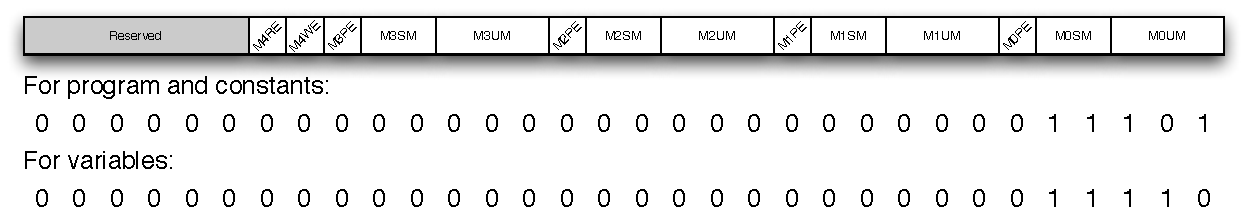
\includegraphics[width=\textwidth]{pictures/MPUprog.pdf} 

So in hexa:

\rowcolors{1}{white}{light-gray}
\begin{longtableii}{l|l}{}{Kind}{Value}
  \lineii{Program region access}
  {$0x00000005$}
  \lineii{Variable region access}
  {$0x0000001E$}
\end{longtableii}

\subsubsection{What happen in case of memory protection violation ?}

Two exception handler are used to handle a memory protection violation, one for data access, one for code access.

The Data Storage exception is tied to the IVOR~2 vector (VPR offset = 0x020), see page 8-2 of the {\em MPC5510 Microcontroller Family Reference Manual}.

The Instruction Storage exception is tied to the IVOR~3 vector (VPR offset = 0x030), see page 8-2 of the {\em MPC5510 Microcontroller Family Reference Manual}.

However, it appears one of these exceptions is raised when the processor is in user mode. The behavior is different in supervisor mode {\em to be completed}.

